\documentclass[aspectratio=169,10pt]{beamer}

\usepackage[T1]{fontenc}
\usepackage[utf8]{inputenc}
\usepackage[brazilian,provide=*]{babel}
\usepackage{lmodern}
\usepackage{textcomp}
\usepackage{booktabs}
\usepackage{array}
\usepackage{listings}
\usepackage{tikz}
\usetikzlibrary{positioning,arrows.meta,fit}

% ---------- estilo: minimalista, preto e cinza ----------
\usefonttheme{serif}
\setbeamersize{text margin left=7mm, text margin right=7mm}
\setbeamertemplate{navigation symbols}{}
\setbeamercolor{structure}{fg=black}
\setbeamercolor{normal text}{fg=black}
\setbeamercolor{frametitle}{fg=black}
\setbeamercolor{title}{fg=black}
\setbeamerfont{frametitle}{size=\large,series=\bfseries}
\setbeamertemplate{itemize item}{\color{black!55}\raisebox{0.15ex}{\scriptsize$\blacksquare$}}
\setbeamertemplate{itemize subitem}{\color{black!45}--}
\setbeamertemplate{footline}{\hfill\color{black!45}\scriptsize\insertframenumber\hspace{1.2em}\vspace{0.8em}}
\setlength{\leftmargini}{1.1em}

\definecolor{cinza}{gray}{0.42}

% ---------- código: cópia literal dos arquivos do trabalho ----------
% Os trechos em trechos/ são gerados por extrai_trechos.py a partir de
% trabalho_final_ferr_comp.R, 03_verificacao.sql e dos blocos P1 a P4.
\lstdefinestyle{codigo}{
  basicstyle=\ttfamily\fontsize{6.5}{7.9}\selectfont,
  columns=fullflexible, keepspaces=true, showstringspaces=false,
  upquote=true, breaklines=true, breakatwhitespace=true,
  frame=leftline, framerule=0.6pt, rulecolor=\color{black!30},
  xleftmargin=0.8em, aboveskip=0.3em, belowskip=0.3em,
  morecomment=[l]{\#}, morestring=[b]", commentstyle=\color{cinza},
  literate={á}{{\'a}}1 {ã}{{\~a}}1 {ê}{{\^e}}1 {í}{{\'i}}1 {ó}{{\'o}}1
           {ú}{{\'u}}1 {Ê}{{\^E}}1 {é}{{\'e}}1 {ç}{{\c{c}}}1 {õ}{{\~o}}1
           {â}{{\^a}}1 {à}{{\`a}}1 {Í}{{\'I}}1 {~}{{\texttildelow}}1}
\lstdefinestyle{codigomenor}{style=codigo,
  basicstyle=\ttfamily\fontsize{6}{7.3}\selectfont}
\lstdefinestyle{codigomaior}{style=codigo,
  basicstyle=\ttfamily\fontsize{7.6}{9.3}\selectfont}
\lstdefinestyle{codigomedio}{style=codigo,
  basicstyle=\ttfamily\fontsize{7}{8.5}\selectfont}
\lstdefinestyle{codigosql}{style=codigo, morecomment=[l]{--}}

\newcommand{\trecho}[2][codigo]{\lstinputlisting[style=#1]{trechos/#2}}
\newcommand{\fonte}[1]{{\scriptsize\color{cinza}#1}}
\newcommand{\cab}[1]{{\small\bfseries #1}\par\vspace{0.3em}}
\newcommand{\cod}[1]{\texttt{#1}}

\title{Uma base de dados relacional da pós-graduação brasileira}
\subtitle{Astronomia/Física e Química nos dados abertos da CAPES (2021--2024)}
\author{Fernando Casellato \quad Felipe Piancatelli\\[0.2em] Ana Carolina Soares \quad Marcos Antônio Garcia}
\institute{Ferramentas Computacionais \\ Docente: Thomas Nogueira Vilches}
\date{}

\begin{document}

% ====================================================================== 1
\begin{frame}[plain]
  \titlepage
\end{frame}

% ====================================================================== 2
\begin{frame}{Contexto}
  \begin{columns}[T]
    \column{0.56\textwidth}
    \begin{itemize}
      \item Um integrante do grupo já trabalhou com os dados da Plataforma Sucupira: 1976 docentes de química, ano de 2016
      \item Naquele estudo o processamento foi todo em R, sem base de dados, e as planilhas eram cruzadas a cada análise
      \item Aqui os dados de 2021 a 2024 de duas áreas de avaliação são organizados em uma base relacional
    \end{itemize}
    \column{0.38\textwidth}
    \vspace{0.6em}
    \begin{block}{}
      \small Casellato, Massi e Nascimento,\\
      \textit{A estrutura interna do campo da química no Brasil},\\
      Química Nova \textbf{48}, e-20250071 (2025)
    \end{block}
  \end{columns}
\end{frame}

% ====================================================================== 3
\begin{frame}{Plataforma Sucupira e dados desagregados}
  \begin{columns}[c]
    \column{0.56\textwidth}
    \centering
    \includegraphics[width=\linewidth]{figuras_v2/figura_dados_abertos_capes.png}
    \column{0.41\textwidth}
    \begin{itemize}
      \item Os programas informam seus dados à CAPES pela Plataforma Sucupira
      \item O portal de Dados Abertos publica um conjunto por tema e um CSV por ano
      \item Programas, Docentes e Discentes, de 2021 a 2024: 12 arquivos, cerca de 1 GB
      \item Uma linha por docente ou discente, com os dados do programa repetidos
      \item O código do programa liga um arquivo ao outro
    \end{itemize}
  \end{columns}
  \vspace{0.4em}
  \fonte{Portal Dados Abertos CAPES, conjunto ``[2021 a 2024] Discentes da Pós-Graduação Stricto Sensu no Brasil''}
\end{frame}

% ====================================================================== 4
\begin{frame}{Objetivo e perguntas}
  \begin{block}{}
    Construir uma base de dados relacional em PostgreSQL com as 12 planilhas e usá-la para comparar os programas acadêmicos de Astronomia/Física e de Química
  \end{block}
  \vspace{0.5em}
  \begin{columns}[T]
    \column{0.64\textwidth}
    \begin{itemize}
      \item[\textbf{P1}] Os programas das duas áreas se distribuem do mesmo modo entre as regiões? A nota dos programas varia entre as regiões?
      \item[\textbf{P2}] A proporção de docentes com bolsa de produtividade do CNPq difere entre as áreas e varia com a nota do programa?
      \item[\textbf{P3}] A proporção de docentes com o último grau obtido no exterior difere entre as áreas e varia com a nota?
      \item[\textbf{P4}] Quantos mestres e doutores cada área titulou de 2021 a 2024, no total e por docente?
    \end{itemize}
    \column{0.31\textwidth}
    \small
    \begin{itemize}
      \item Só programas acadêmicos
      \item Docentes permanentes e colaboradores
      \item Nota: Avaliação Quadrienal 2017--2020
      \item P1 a P3: ano de 2024
    \end{itemize}
  \end{columns}
\end{frame}

% ====================================================================== 5
\begin{frame}{Etapas do processamento}
  \centering
  \vspace{1em}
  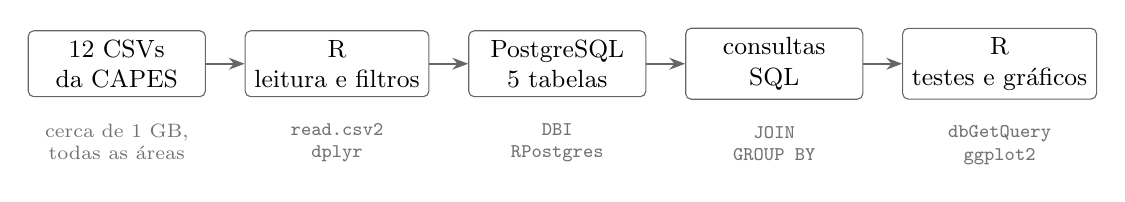
\begin{tikzpicture}[
      caixa/.style={draw=black!60, rounded corners=2pt, minimum height=2.2em,
                    minimum width=6.4em, align=center, font=\small},
      seta/.style={-{Stealth[length=2mm]}, black!60, thick},
      nota/.style={font=\scriptsize, text=black!55, align=center}]
    \node[caixa] (csv) {12 CSVs\\da CAPES};
    \node[caixa, right=1.4em of csv] (r1) {R\\leitura e filtros};
    \node[caixa, right=1.4em of r1] (pg) {PostgreSQL\\5 tabelas};
    \node[caixa, right=1.4em of pg] (sql) {consultas\\SQL};
    \node[caixa, right=1.4em of sql] (r2) {R\\testes e gráficos};
    \draw[seta] (csv) -- (r1);
    \draw[seta] (r1) -- (pg);
    \draw[seta] (pg) -- (sql);
    \draw[seta] (sql) -- (r2);
    \node[nota, below=0.6em of csv] {cerca de 1 GB,\\todas as áreas};
    \node[nota, below=0.6em of r1] {\texttt{read.csv2}\\\texttt{dplyr}};
    \node[nota, below=0.6em of pg] {\texttt{DBI}\\\texttt{RPostgres}};
    \node[nota, below=0.6em of sql] {\texttt{JOIN}\\\texttt{GROUP BY}};
    \node[nota, below=0.6em of r2] {\texttt{dbGetQuery}\\\texttt{ggplot2}};
  \end{tikzpicture}

  \vspace{2em}
  \begin{itemize}
    \item As cinco etapas estão em um arquivo, \texttt{trabalho\_final\_ferr\_comp.R}
    \item Cada pergunta é um bloco de código acrescentado ao fim desse arquivo
  \end{itemize}
\end{frame}

% ====================================================================== 6
\begin{frame}{Tabelas de referência e tabelas de dados}
  \centering
  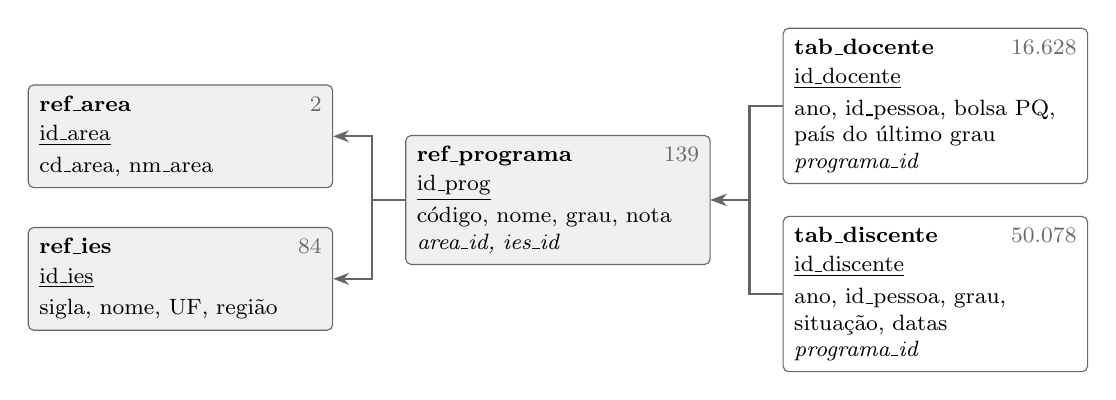
\begin{tikzpicture}[
      tab/.style={draw=black!60, rounded corners=2pt, align=left, font=\footnotesize,
                  inner sep=4pt, text width=10.2em},
      ref/.style={tab, fill=black!6},
      fk/.style={-{Stealth[length=2mm]}, black!60, thick}]
    \node[ref] (area) {\textbf{ref\_area}\hfill\textcolor{cinza}{2}\\[1pt]
      \underline{id\_area}\\[2pt] cd\_area, nm\_area};
    \node[ref, below=1.4em of area] (ies) {\textbf{ref\_ies}\hfill\textcolor{cinza}{84}\\[1pt]
      \underline{id\_ies}\\[2pt] sigla, nome, UF, região};
    \node[ref, right=2.6em of area, yshift=-2.3em] (prog) {\textbf{ref\_programa}\hfill\textcolor{cinza}{139}\\[1pt]
      \underline{id\_prog}\\[2pt] código, nome, grau, nota\\ \textit{area\_id, ies\_id}};
    \node[tab, right=2.6em of prog, yshift=3.4em] (doc) {\textbf{tab\_docente}\hfill\textcolor{cinza}{16.628}\\[1pt]
      \underline{id\_docente}\\[2pt] ano, id\_pessoa, bolsa PQ,\\ país do último grau\\ \textit{programa\_id}};
    \node[tab, right=2.6em of prog, yshift=-3.4em] (disc) {\textbf{tab\_discente}\hfill\textcolor{cinza}{50.078}\\[1pt]
      \underline{id\_discente}\\[2pt] ano, id\_pessoa, grau,\\ situação, datas\\ \textit{programa\_id}};
    \draw[fk] (prog.west) -- ++(-1.2em,0) |- (area.east);
    \draw[fk] (prog.west) -- ++(-1.2em,0) |- (ies.east);
    \draw[fk] (doc.west) -- ++(-1.2em,0) |- (prog.east);
    \draw[fk] (disc.west) -- ++(-1.2em,0) |- (prog.east);
  \end{tikzpicture}

  \vspace{0.8em}
  \begin{columns}[T]
    \column{0.46\textwidth}
    \begin{itemize}
      \item \colorbox{black!6}{Referência}: cada área, instituição e programa em uma única linha
      \item Dados: uma linha por docente ou discente em cada programa e ano
    \end{itemize}
    \column{0.46\textwidth}
    \begin{itemize}
      \item \underline{Sublinhado}: chave primária
      \item \textit{Itálico} e setas: chaves estrangeiras
      \item À direita do nome: número de linhas
    \end{itemize}
  \end{columns}
\end{frame}

% ====================================================================== 7
\begin{frame}{Chaves primárias e estrangeiras}
  \trecho[codigomedio]{base_chaves.R}
  \vspace{0.6em}
  \begin{columns}[T]
    \column{0.47\textwidth}
    \begin{itemize}
      \item \cod{id\_prog} é a chave primária, numerada pelo próprio banco
      \item \cod{UNIQUE} impede que o mesmo código da CAPES entre duas vezes
    \end{itemize}
    \column{0.47\textwidth}
    \begin{itemize}
      \item \cod{area\_id} e \cod{ies\_id} são chaves estrangeiras para \cod{ref\_area} e \cod{ref\_ies}
      \item O banco recusa um programa que aponte para uma área ou instituição inexistente
    \end{itemize}
  \end{columns}
\end{frame}

% ====================================================================== 8
\begin{frame}{Leitura e filtragem dos CSVs}
  \trecho[codigomaior]{base_leitura.R}
  \vspace{0.6em}
  \begin{columns}[T]
    \column{0.47\textwidth}
    \begin{itemize}
      \item \cod{read.csv2} lê o separador ponto e vírgula; os arquivos da CAPES estão em latin1
      \item Tudo é lido como texto para os códigos não perderem dígitos
    \end{itemize}
    \column{0.47\textwidth}
    \begin{itemize}
      \item \cod{filter} roda logo após a leitura de cada arquivo: ficam as duas áreas e os programas acadêmicos
      \item \cod{bind\_rows} empilha os quatro anos de um tema
    \end{itemize}
  \end{columns}
\end{frame}

% ====================================================================== 9
\lstdefinestyle{codigocarga}{style=codigo,
  basicstyle=\ttfamily\fontsize{6.2}{7.5}\selectfont}
\begin{frame}{Carga no PostgreSQL}
  \trecho[codigocarga]{base_trocar_id.R}
  \trecho[codigocarga]{base_gravar.R}
  \trecho[codigocarga]{base_docente.R}
  \small
  \begin{columns}[T]
    \column{0.47\textwidth}
    \begin{itemize}
      \item \cod{trocar\_id}: um \cod{left\_join} com a tabela de referência troca o código da CAPES pelo identificador da base
    \end{itemize}
    \column{0.47\textwidth}
    \begin{itemize}
      \item \cod{dbWriteTable} com \cod{append = TRUE} acrescenta as linhas à tabela já criada
      \item As tabelas de referência são carregadas antes das de dados
    \end{itemize}
  \end{columns}
\end{frame}

% ====================================================================== 10
\begin{frame}{Consultas com JOIN}
  \begin{columns}[T]
    \column{0.49\textwidth}
    \trecho[codigosql]{base_consulta.sql}
    \vspace{0.8em}
    \begin{itemize}
      \item Dois \cod{JOIN} levam de cada docente ao programa e do programa à área
      \item Em 2024, Astronomia/Física tem 1881 vínculos e 1775 docentes distintos: quem atua em dois programas ocupa duas linhas
    \end{itemize}
    \column{0.48\textwidth}
    \centering\scriptsize\setlength{\tabcolsep}{3.2pt}
    \begin{tabular}{@{}llrrr@{}}
      \toprule
      ano & área & programas & vínculos & docentes \\
      \midrule
      2021 & Astronomia/Física & 64 & 1854 & 1749 \\
      2021 & Química           & 73 & 2328 & 2140 \\
      2022 & Astronomia/Física & 61 & 1850 & 1754 \\
      2022 & Química           & 71 & 2304 & 2147 \\
      2023 & Astronomia/Física & 64 & 1893 & 1778 \\
      2023 & Química           & 71 & 2275 & 2124 \\
      2024 & Astronomia/Física & 62 & 1881 & 1775 \\
      2024 & Química           & 72 & 2243 & 2092 \\
      \bottomrule
    \end{tabular}

    \vspace{0.6em}
    \fonte{Resultado da consulta. Docentes: \cod{COUNT(DISTINCT id\_pessoa)}}
  \end{columns}
\end{frame}

% ====================================================================== 11
\begin{frame}{Unidade de análise e leitura dos testes}
  \begin{columns}[T]
    \column{0.50\textwidth}
    \begin{itemize}
      \item Região e nota são atributos do programa, repetidos em todos os seus docentes
      \item Docentes de um mesmo programa não são observações independentes
      \item Os testes e os modelos usam o programa como observação
      \item A base contém todos os programas das duas áreas: o p-valor compara a diferença observada com a variação entre programas, sem erro de amostragem envolvido
      \item As relações encontradas são associações
    \end{itemize}
    \column{0.46\textwidth}
    \cab{Área $\times$ região, 2024}
    \footnotesize\setlength{\tabcolsep}{2.8pt}
    \begin{tabular}{@{}lrlr@{}}
      \toprule
      observação & $n$ & teste & $p$ \\
      \midrule
      vínculo de docente & 4124 & qui-quadrado & $<0{,}001$ \\
      programa & 134 & exato de Fisher & $0{,}28$ \\
      \bottomrule
    \end{tabular}

    \vspace{0.8em}
    \begin{itemize}
      \item Com os docentes como observações, $\chi^2 = 121{,}1$ (4 graus de liberdade)
      \item O mesmo cruzamento com os 134 programas não rejeita a hipótese de distribuições iguais
    \end{itemize}
  \end{columns}
\end{frame}

% ====================================================================== 12
\begin{frame}{P1 $\cdot$ Consulta e testes}
  \begin{columns}[T]
    \column{0.64\textwidth}
    \trecho{p1_consulta.R}
    \trecho{p1_fisher.R}
    \trecho{p1_wilcox.R}
    \trecho{p1_kruskal.R}
    \column{0.32\textwidth}
    \small
    \begin{itemize}
      \item \cod{GROUP BY}: uma linha por programa com docentes em 2024
      \item Fisher: tabela área $\times$ região, com células de 2 a 4 programas
      \item Mann-Whitney: nota comparada entre as duas áreas
      \item Kruskal-Wallis: nota comparada entre as cinco regiões
      \item A nota entra como escala ordenada, sem supor normalidade
    \end{itemize}
  \end{columns}
\end{frame}

% ====================================================================== 13
\begin{frame}{P1 $\cdot$ Programas e docentes por região}
  \begin{columns}[c]
    \column{0.65\textwidth}
    \includegraphics[width=\linewidth]{figuras_v2/P1_programas_docentes_por_regiao.pdf}
    \column{0.32\textwidth}
    \small
    \begin{itemize}
      \item Sudeste: 32 dos 62 programas de Astronomia/Física (52\%) e 25 dos 72 de Química (35\%)
      \item Fisher sobre os programas: $p = 0{,}28$
      \item Uma diferença desse tamanho é comum quando área e região não têm relação
      \item Docentes no Sudeste: 60\% e 45\%, apresentados como descrição
    \end{itemize}
  \end{columns}
\end{frame}

% ====================================================================== 14
\begin{frame}{P1 $\cdot$ Gráfico da nota por região}
  \begin{columns}[T]
    \column{0.64\textwidth}
    \trecho{p1_ggplot.R}
    \column{0.32\textwidth}
    \small
    \begin{itemize}
      \item \cod{geom\_col}: barras empilhadas com o número de programas
      \item \cod{p1\_cinzas}: a nota é uma categoria ordenada e recebe uma escala de cinzas
      \item \cod{position\_stack}: o número de programas no centro de cada segmento
      \item \cod{facet\_wrap}: um painel por área
    \end{itemize}
  \end{columns}
\end{frame}

% ====================================================================== 15
\begin{frame}{P1 $\cdot$ Nota dos programas por região}
  \begin{columns}[c]
    \column{0.65\textwidth}
    \includegraphics[width=\linewidth]{figuras_v2/P1_nota_por_regiao.pdf}
    \column{0.32\textwidth}
    \small
    \begin{itemize}
      \item Nota 6 ou 7: 21 de 55 programas no Sudeste (38\%) e 4 de 30 no Nordeste (13\%)
      \item Kruskal-Wallis com as duas áreas: $H = 15{,}3$, $p = 0{,}004$
      \item Por área: $p = 0{,}003$ na Química e $p = 0{,}49$ em Astronomia/Física
      \item Astronomia/Física tem 2 programas no Norte e 3 no Centro-Oeste
      \item Nota entre as áreas: medianas 5 e 4, Mann-Whitney $p = 0{,}16$
    \end{itemize}
  \end{columns}
\end{frame}

% ====================================================================== 16
\begin{frame}{Síntese da P1}
  \begin{columns}[T]
    \column{0.47\textwidth}
    \cab{Os dados mostram}
    \begin{itemize}
      \item Com 134 programas, a diferença regional entre as áreas não se distingue da variação casual
      \item A nota está associada à região: o Sudeste tem 42\% dos programas avaliados e 57\% dos de nota 6 ou 7
      \item Nas duas áreas, 28\% dos programas têm nota 6 ou 7
    \end{itemize}
    \column{0.47\textwidth}
    \cab{Os dados não permitem afirmar}
    \begin{itemize}
      \item Que a relação entre nota e região exista só na Química: um teste significativo e outro não significativo não comparam as áreas entre si
      \item Por que a nota varia entre as regiões
      \item Algo sobre o acesso das pessoas à pós-graduação: a base não registra a origem de docentes e discentes
    \end{itemize}
  \end{columns}
\end{frame}

% ====================================================================== 17
\begin{frame}{P2 $\cdot$ Consulta e modelo}
  \begin{columns}[T]
    \column{0.64\textwidth}
    \trecho{p2_consulta.R}
    \trecho{p2_prog.R}
    \trecho{p2_modelo.R}
    \trecho{p2_interacao.R}
    \column{0.32\textwidth}
    \small
    \begin{itemize}
      \item \cod{DISTINCT ON}: cada docente conta uma vez por área e ano, no programa de nota mais alta
      \item \cod{cbind}: a resposta são os bolsistas e os não bolsistas de cada programa
      \item \cod{quasibinomial}: erros-padrão corrigidos pela variação entre programas
      \item \cod{anova} com teste F: o efeito da nota é o mesmo nas duas áreas?
    \end{itemize}
  \end{columns}
\end{frame}

% ====================================================================== 18
\begin{frame}{P2 $\cdot$ Gráfico por programa}
  \begin{columns}[T]
    \column{0.64\textwidth}
    \trecho{p2_ggplot.R}
    \column{0.32\textwidth}
    \small
    \begin{itemize}
      \item \cod{geom\_point}: um ponto por programa, com deslocamento lateral para não sobrepor
      \item \cod{geom\_errorbar} com \cod{ymin = ymax}: um traço no percentual do conjunto de docentes da área e da nota
      \item \cod{cores\_area}: cada área tem a mesma cor em todos os gráficos
    \end{itemize}
  \end{columns}
\end{frame}

% ====================================================================== 19
\begin{frame}{P2 $\cdot$ Bolsistas de produtividade por nota do programa}
  \begin{columns}[c]
    \column{0.63\textwidth}
    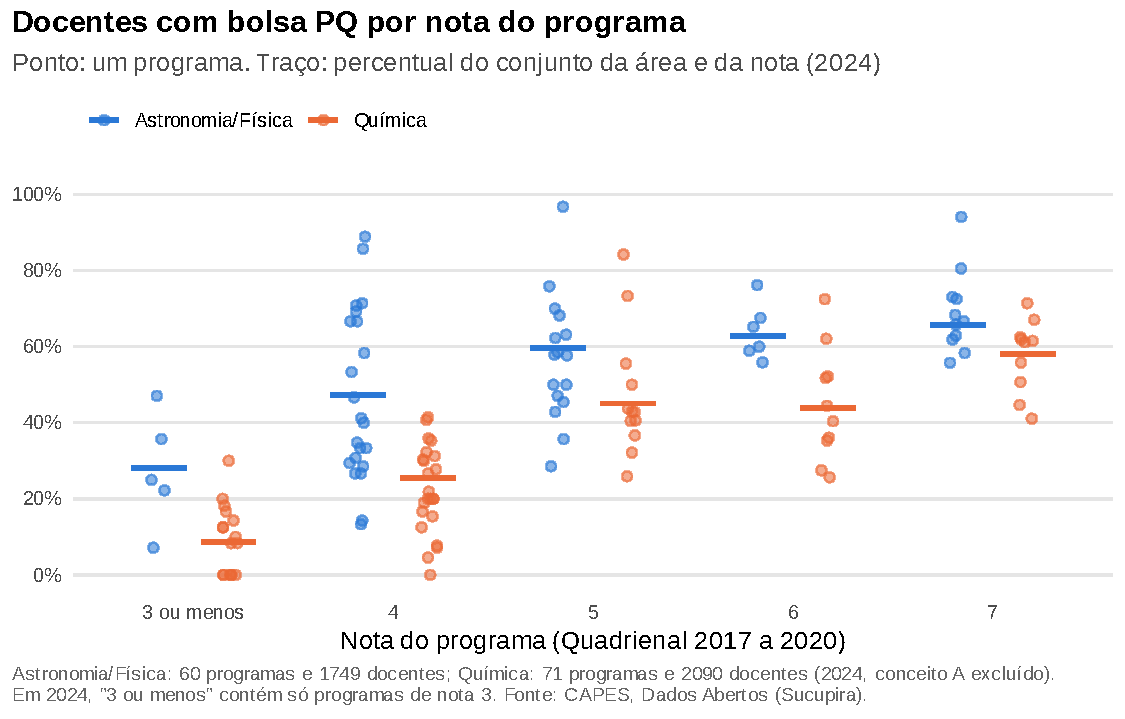
\includegraphics[width=\linewidth]{figuras_v2/P2_pq_por_nota_programas.pdf}
    \column{0.34\textwidth}
    \small
    \begin{itemize}
      \item 2024: 58,0\% dos docentes de Astronomia/Física e 39,4\% dos de Química têm bolsa
      \item Da nota 3 à nota 7: de 28\% a 66\% e de 9\% a 58\%
      \item Entre os programas: de 7\% a 97\% e de 0\% a 84\%
      \item Programas de mesma área e mesma nota diferem em dezenas de pontos percentuais
    \end{itemize}
  \end{columns}
\end{frame}

% ====================================================================== 20
\begin{frame}{P2 $\cdot$ Regressão logística sobre os programas}
  \begin{columns}[T]
    \column{0.50\textwidth}
    \small
    \begin{tabular}{@{}lcc@{}}
      \toprule
      termo & razão de chances & IC 95\% \\
      \midrule
      Química & 0,52 & 0,42 a 0,64 \\
      nota 3  & 0,33 & 0,19 a 0,58 \\
      nota 5  & 2,00 & 1,48 a 2,69 \\
      nota 6  & 2,06 & 1,49 a 2,84 \\
      nota 7  & 3,00 & 2,28 a 3,94 \\
      \bottomrule
    \end{tabular}

    \vspace{0.6em}
    \fonte{Referência: Astronomia/Física, nota 4. 131 programas e 3839 docentes.\\
           Dispersão estimada: 2,32.}
    \column{0.46\textwidth}
    \small
    \begin{itemize}
      \item Nota como tendência linear: razão de chances de 1,49 por ponto (IC 95\% de 1,37 a 1,61)
      \item Notas 5 e 6 têm razões quase iguais
      \item Interação área $\times$ nota: $p = 0{,}10$ com a nota em categorias e $p = 0{,}006$ com a nota como tendência
      \item Tendência em cada área: 1,31 por ponto em Astronomia/Física e 1,65 em Química
    \end{itemize}
  \end{columns}
\end{frame}

% ====================================================================== 21
\begin{frame}{Síntese da P2}
  \begin{columns}[T]
    \column{0.47\textwidth}
    \cab{Os dados mostram}
    \begin{itemize}
      \item Em programas de mesma nota, a bolsa de produtividade é menos frequente na Química (razão de chances 0,52)
      \item A proporção de bolsistas cresce com a nota nas duas áreas
      \item De 2021 a 2024 os percentuais ficaram entre 57\% e 58\% em Astronomia/Física e entre 39\% e 40\% na Química
    \end{itemize}
    \column{0.47\textwidth}
    \cab{Os dados não permitem afirmar}
    \begin{itemize}
      \item Que a nota atraia bolsas ou que as bolsas elevem a nota: a Quadrienal 2017--2020 avaliou em parte a produção desses mesmos docentes
      \item Que a diferença entre as áreas meça desempenho: as bolsas são distribuídas por área no CNPq
      \item Que o aumento com a nota seja mais forte na Química: o resultado muda com a forma de incluir a nota no modelo
    \end{itemize}
  \end{columns}
\end{frame}

% ====================================================================== 22
\begin{frame}{P3 $\cdot$ Variável, modelo e gráfico dos países}
  \begin{columns}[T]
    \column{0.42\textwidth}
    \trecho[codigomenor]{p3_variavel.R}
    \trecho[codigomenor]{p3_prog.R}
    \trecho[codigomenor]{p3_modelo.R}
    \column{0.55\textwidth}
    \trecho[codigomenor]{p3_ggplot.R}
  \end{columns}
  \vspace{0.5em}
  \begin{itemize}
    \item \cod{exterior}: o país da instituição do último grau do docente é diferente de Brasil
    \item O modelo tem a mesma forma do usado na P2, com os titulados no exterior no lugar dos bolsistas
  \end{itemize}
\end{frame}

% ====================================================================== 23
\begin{frame}{P3 $\cdot$ Último grau no exterior por nota do programa}
  \begin{columns}[c]
    \column{0.63\textwidth}
    \includegraphics[width=\linewidth]{figuras_v2/P3_exterior_por_nota_programas.pdf}
    \column{0.34\textwidth}
    \small
    \begin{itemize}
      \item 2024: 22,3\% dos docentes de Astronomia/Física (390 de 1749) e 8,6\% dos de Química (179 de 2090)
      \item Razão de chances da Química: 0,36 (IC 95\% de 0,28 a 0,46)
      \item Por ponto de nota: 1,37 (1,25 a 1,50)
      \item Interação área $\times$ nota: $p = 0{,}52$ em categorias e $p = 0{,}14$ como tendência
      \item Dispersão estimada: 1,55
    \end{itemize}
  \end{columns}
\end{frame}

% ====================================================================== 24
\begin{frame}{P3 $\cdot$ País do último grau}
  \begin{columns}[c]
    \column{0.60\textwidth}
    \includegraphics[width=\linewidth]{figuras_v2/P3_paises_titulacao.pdf}
    \column{0.37\textwidth}
    \small
    \begin{itemize}
      \item Estados Unidos, França e Reino Unido somam 195 docentes de Astronomia/Física (11,1\%) e 97 de Química (4,6\%)
      \item Na Química a França vem antes dos Estados Unidos: 39 e 31 docentes
      \item Os percentuais são sobre todos os docentes de cada área
    \end{itemize}
  \end{columns}
\end{frame}

% ====================================================================== 25
\begin{frame}{Síntese da P3}
  \begin{columns}[T]
    \column{0.47\textwidth}
    \cab{Os dados mostram}
    \begin{itemize}
      \item O último grau no exterior é mais frequente em Astronomia/Física em todas as notas
      \item A proporção cresce com a nota, sem evidência de que o crescimento difira entre as áreas
      \item De 2021 a 2024 os percentuais ficaram perto de 22\% em Astronomia/Física e de 9\% na Química
    \end{itemize}
    \column{0.47\textwidth}
    \cab{Os dados não permitem afirmar}
    \begin{itemize}
      \item Quantos docentes tiveram experiência no exterior: doutorado sanduíche e pós-doutorado não estão na base
      \item Quantos são brasileiros que se titularam fora e quantos são estrangeiros contratados no Brasil
      \item Que a titulação no exterior explique a nota do programa
    \end{itemize}
  \end{columns}
\end{frame}

% ====================================================================== 26
\begin{frame}{P4 $\cdot$ Gráfico dos titulados por ano}
  \begin{columns}[T]
    \column{0.64\textwidth}
    \trecho{p4_ggplot.R}
    \column{0.32\textwidth}
    \small
    \begin{itemize}
      \item \cod{geom\_line} e \cod{geom\_point}: uma série por área
      \item \cod{facet\_wrap}: um painel para o mestrado e outro para o doutorado
      \item O segundo \cod{geom\_text} escreve o nome da área no fim da linha e dispensa a legenda
      \item O eixo vertical começa em zero
    \end{itemize}
  \end{columns}
\end{frame}

% ====================================================================== 27
\begin{frame}{P4 $\cdot$ Titulados por ano}
  \begin{columns}[c]
    \column{0.65\textwidth}
    \includegraphics[width=\linewidth]{figuras_v2/P4_titulados_por_ano.pdf}
    \column{0.32\textwidth}
    \small
    \begin{itemize}
      \item Astronomia/Física: 2222 mestres e 1511 doutores no quadriênio
      \item Química: 3461 mestres e 2609 doutores
      \item A Química titulou 1,56 vez o número de mestres e 1,73 vez o de doutores
      \item A Química também tem mais programas (74 e 65) e mais docentes
    \end{itemize}
  \end{columns}
\end{frame}

% ====================================================================== 28
\begin{frame}{P4 $\cdot$ Consulta por programa e modelo}
  \begin{columns}[T]
    \column{0.62\textwidth}
    \trecho{p4_consulta.R}
    \trecho{p4_modelo.R}
    \column{0.34\textwidth}
    \small
    \begin{itemize}
      \item \cod{WITH}: duas subconsultas agregadas por programa
      \item Docentes-ano: soma dos docentes do programa nos quatro anos
      \item \cod{LEFT JOIN} e \cod{COALESCE}: programa sem titulados entra com zero
      \item \cod{offset}: o modelo descreve titulados por docente por ano
      \item \cod{quasipoisson}: erros-padrão corrigidos pela variação entre programas
    \end{itemize}
  \end{columns}
\end{frame}

% ====================================================================== 29
\begin{frame}{P4 $\cdot$ Titulados por docente por ano}
  \begin{columns}[c]
    \column{0.67\textwidth}
    \includegraphics[width=\linewidth]{figuras_v2/P4_titulados_por_docente.pdf}
    \column{0.30\textwidth}
    \small
    \begin{itemize}
      \item Doutores por docente por ano: 0,23 em Astronomia/Física e 0,33 na Química
      \item Mestres: 0,30 e 0,40
      \item Razão de taxas da Química: 1,49 para doutores (IC 95\% de 1,25 a 1,78) e 1,29 para mestres (1,15 a 1,45)
      \item Doutores, interação área $\times$ nota: $p = 0{,}029$
      \item Doutores na nota 4: 0,23 e 0,22; na nota 7: 0,22 e 0,42
    \end{itemize}
  \end{columns}
\end{frame}

% ====================================================================== 30
\begin{frame}{Síntese da P4}
  \begin{columns}[T]
    \column{0.47\textwidth}
    \cab{Os dados mostram}
    \begin{itemize}
      \item A Química titulou mais mestres e mais doutores no quadriênio, em número absoluto e por docente
      \item No doutorado, a diferença por docente aparece nos programas de nota 5 a 7
      \item Em Astronomia/Física a taxa de doutores fica entre 0,22 e 0,25 em todas as notas
    \end{itemize}
    \column{0.47\textwidth}
    \cab{Os dados não permitem afirmar}
    \begin{itemize}
      \item Que a taxa meça eficiência: ela não considera quantos discentes ingressaram nem o tempo até a titulação
      \item Que programas só de mestrado e programas com doutorado sejam comparáveis: o denominador é o corpo docente inteiro nos dois casos
      \item Como se comportam os doutorados recentes: 2 programas de Química com doutorado não titularam doutores no período
    \end{itemize}
  \end{columns}
\end{frame}

% ====================================================================== 31
\begin{frame}{Resultados e limitações}
  \small
  \begin{tabular}{@{}l>{\raggedright\arraybackslash}p{0.88\textwidth}@{}}
    \toprule
    \textbf{P1} & A distribuição regional dos programas não difere de forma detectável entre as áreas ($p = 0{,}28$). A nota varia entre as regiões ($p = 0{,}004$). \\
    \addlinespace
    \textbf{P2} & Em programas de mesma nota, a bolsa de produtividade é menos frequente na Química (razão de chances 0,52) e cresce com a nota (1,49 por ponto). \\
    \addlinespace
    \textbf{P3} & O último grau no exterior é menos frequente na Química (razão de chances 0,36) e cresce com a nota (1,37 por ponto). \\
    \addlinespace
    \textbf{P4} & A Química titulou 3461 mestres e 2609 doutores; Astronomia/Física, 2222 e 1511. Por docente, a razão de taxas é 1,29 para mestres e 1,49 para doutores. \\
    \bottomrule
  \end{tabular}

  \vspace{0.9em}
  \begin{columns}[T]
    \column{0.47\textwidth}
    \begin{itemize}
      \item Os dados são informados pelos próprios programas à CAPES
      \item Há uma única avaliação no período, a de 2017--2020
    \end{itemize}
    \column{0.47\textwidth}
    \begin{itemize}
      \item Norte e Centro-Oeste somam 18 dos 131 programas com nota
      \item A base não registra a produção, a trajetória nem a origem das pessoas
    \end{itemize}
  \end{columns}
\end{frame}

\end{document}
